\section{Section 5.  Project \char`\"{}Big Picture\char`\"{}}\label{page_big_picture}
 \begin{Desc}
\item[Section 5.1.  Covered Big Picture]\par
 The following diagram illustrates the various core functions of Covered and how they are integrated into the tool.\end{Desc}
 \begin{figure}[H]
\begin{center}
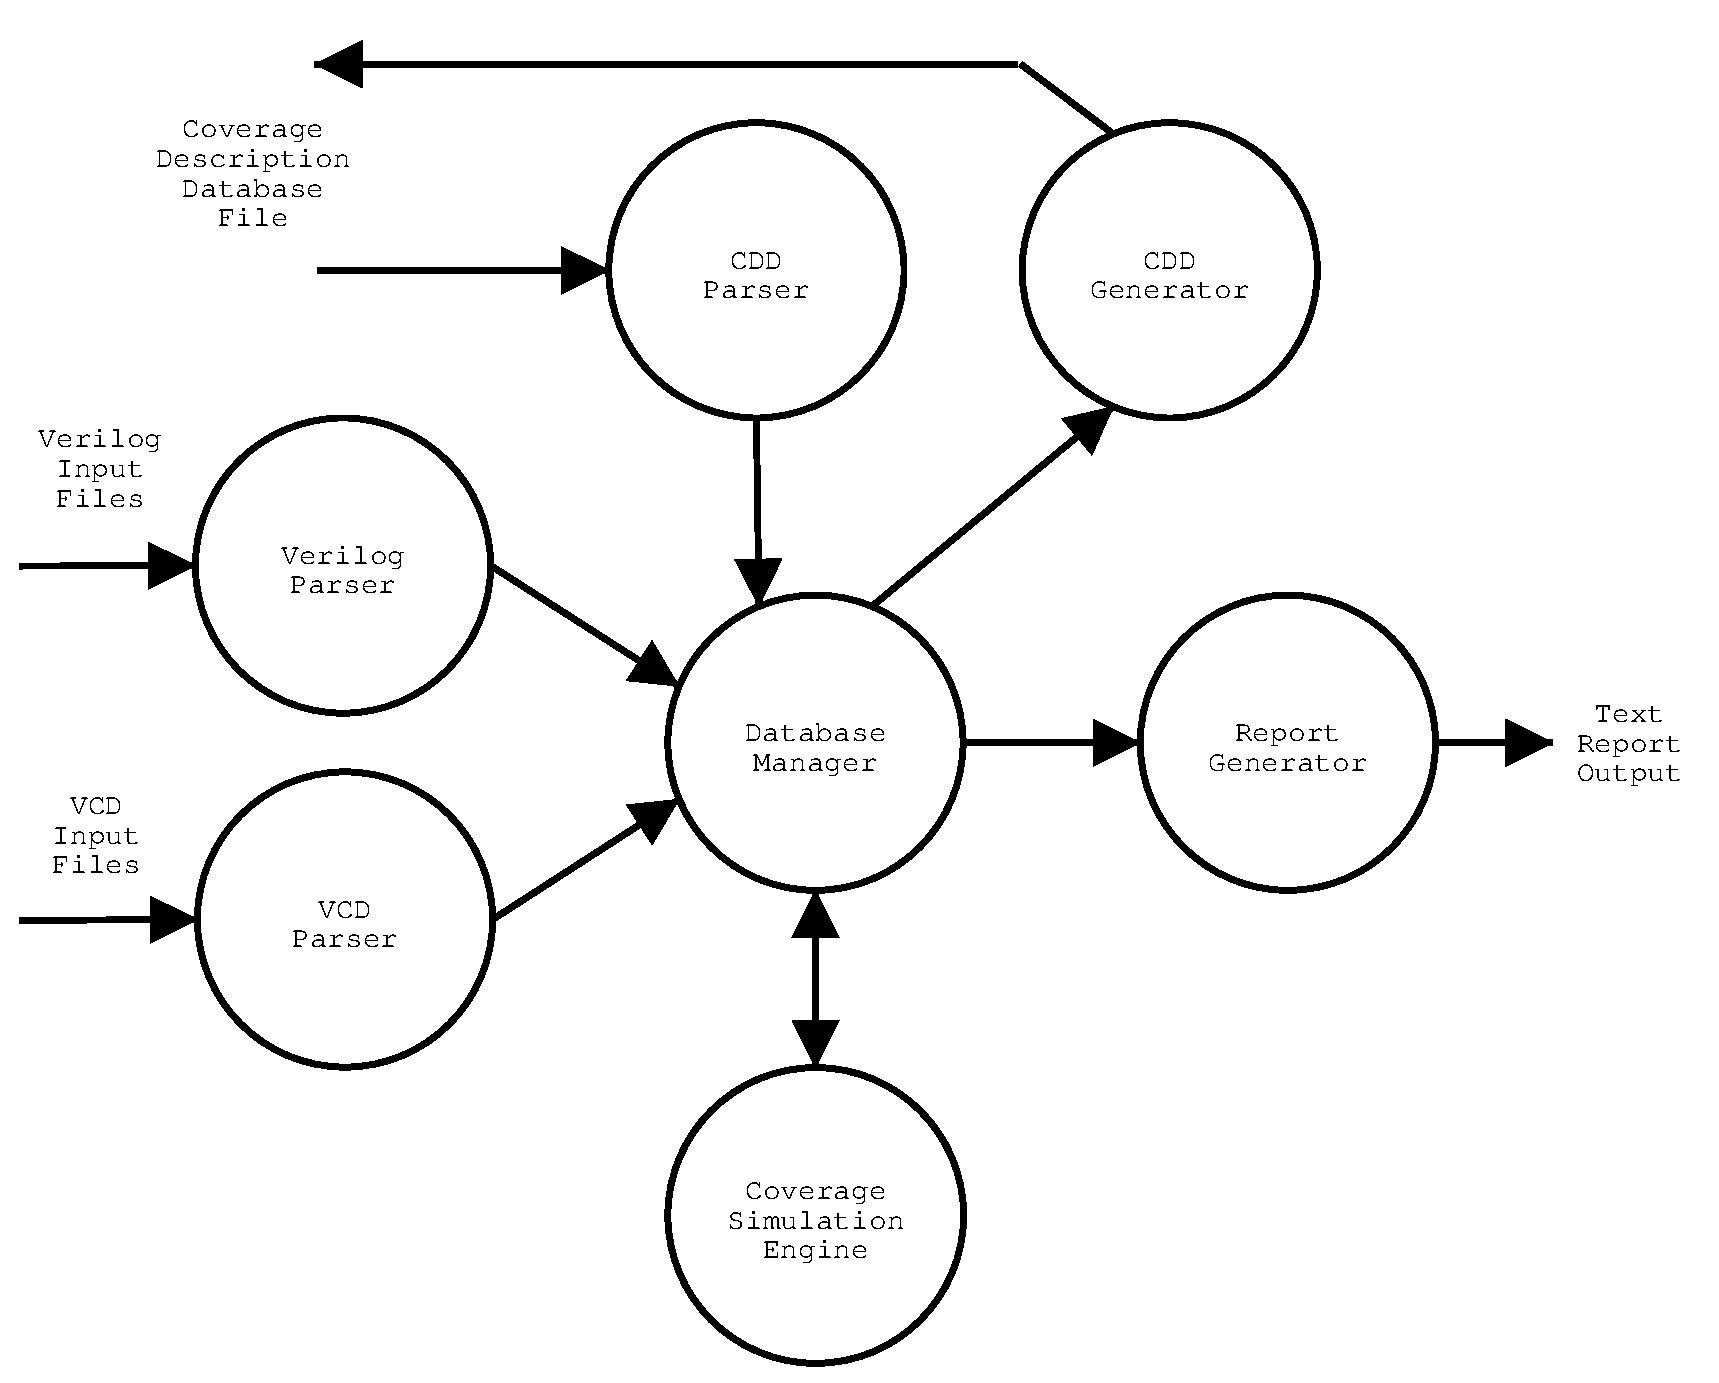
\includegraphics{big_picture.eps}\caption{Figure 1.  Data Flow Diagram}
\end{center}
\end{figure}
 

\begin{Desc}
\item[Section 5.2.  Functional Block Descriptions]\par
 The following subsections describes each of these functions/nodes in greater detail.\end{Desc}
\begin{Desc}
\item[Section 5.2.1.  Verilog Parser]\par
 The Verilog parser used by Covered consists of a Flex lexical analyzer lexer.l and  Bison parser parser.y . Both the lexer and parser where used from the Icarus Verilog project which can be accessed at

 {\tt http://icarus.com/eda/verilog/index.html}

 Though most of the structure of both of these files maintain their original appearance from the Icarus project, most of the internal rule code has been removed and re-implemented to suite Covered's needs from the parser. The parser and lexer work together as most language parsers do with the lexer reading in tokens of information from the input files and passing these tokens for the parser to match with pre-existing language rules. The reason for taking both the lexer and parser from the Icarus project is that the Icarus project is well-used by the g\-EDA community for Verilog simulation and passes in regression the IV testsuite. This testsuite is part of the Verilog testsuite for Covered and is available for download at

 {\tt http://ivtest.sourceforge.net}

 Using the Verilog directory and file pathnames specified on the command-line, Covered generates a list of files to search for Verilog module names. The first module name that Covered attempts to find is the top-level module targetted for coverage. This module name is also specified on the command-line with the {\tt -t} option. The lexer reads in the file and finds the name specified after the Verilog {\bf keyword} {\rm (p.\,\pageref{structkeyword})} {\tt {\bf module}}. If this module matches the top-level module name, the contents of the module are parsed. If the module name does not match the top-level module name, the lexer skips the body of the module until it  encounters the {\tt endmodule} {\bf keyword} {\rm (p.\,\pageref{structkeyword})}. If there are any more modules specified in the given file, these are parsed in the same fashion. If the end of the file has been reached and no module has been found that is needed, the Verilog file is placed at the end of the file  queue and the next file at the head of the queue is read in by the lexer.

 If the top-level module contains module instantiations that also need to be tested for coverage, these module names are placed at the tail of the needed module queue. When the needed module queue is empty, all modules have been found and parsed, and the parsing phase of the procedure is considered complete and successful.

 When the parser finds a match for one of its rules, an action is taken. This action is typically one of the following:

\begin{enumerate}
\item 
Create a new structure for data storage.\item 
Store a structure into one of the lists or trees for later retrieval.\item 
Manipulate a structure based on some information parsed.\item 
Display an error message due to finding code that is incorrect language structure.\end{enumerate}
\end{Desc}


 The Verilog parser only sends information to and gets information from the database manager. When parsing is complete, the database manager contains all of the information from the Verilog design which is stored in special containers which are organized by a group of trees and lists.



\begin{Desc}
\item[Section 5.2.2.  Database Manager]\par
 {\bf TBD}\end{Desc}


\begin{Desc}
\item[Section 5.2.3.  CDD Parser]\par
 The Coverage Description Database file, or CDD as it is referred to in this documentation, is a generalized description of a Verilog design that contains coverage-specific information as it pertains to that design. CDD files are in ASCII text format. The reasons for having this file format are three-fold.

\begin{enumerate}
\item 
Allow a way to store information about a particular design in a way that is compact and concise. It is understood that a CDD file may exist for an indeterminant amount of time so it is important that the file size be as small as possible while still carrying enough information to generate useful coverage reports.\item 
Create a standardized output format that is easy to parse (can be done with the sscanf utility in a straight-forward way) not requiring the use and overhead of another lexer  and parser. The standardization of the file format allows several CDDs to be easily merged and output in the same format.\item 
Create a format that is flexible enough to add new constructs as needed to support the growing Verilog language while not making it more difficult to parse.\end{enumerate}
\end{Desc}


 The generic output format for the CDD file is as follows:

 {\tt $<$unique\_\-numeric\_\-ID\_\-for\_\-construct$>$} {\tt $<$information\_\-about\_\-construct\_\-separated\_\-by\_\-spaces$>$}

 If a new construct needs to be added to the tool, one merely needs to select a unique ID for that construct and come up with a format for displaying the information for that construct so that it is separated by spaces or commas and contains only one ENDLINE character at the end of the line. Blank lines or comments are allowed within the file. The current constructs that are output to a CDD file by Covered are listed below along with their unique ID.

\begin{CompactItemize}
\item 
signal (1)\item 
expression (2)\item 
module (3)\item 
statement (4)\end{CompactItemize}


 The information format for each construct is listed with the description of the construct in the {\bf Section 6.  Coverage Development Reference} {\rm (p.\,\pageref{page_code_details})} section.

 Each line of the CDD file is read into memory by the CDD parser and the first value of the line (the unique construct ID) is used to call the {\tt db\_\-read} function of the associated construct. The construct then takes the initiative of decoding the rest of the line and storing its contents into the same set of lists and trees that the Verilog parser stores its information into. The end result of parsing in the CDD file is the same as parsing in a design by the Verilog parser. Once into memory, the information can be merged, simulated, or computed on by the report generator.



\begin{Desc}
\item[Section 5.2.4.  CDD Generator]\par
 The CDD generator is actually distributed among the various constructs that make up the CDD file. The main {\tt db\_\-write} function located in {\bf db.c} calls each of the construct's {\tt db\_\-write} functions which, in turn, output their information to the CDD file in their own format. After each of the stored constructs have written their information to the CDD file, it is closed by the {\tt db\_\-write} function. The end result is a CDD file that is in the same format as the CDD file that was read in by the CDD parser.\end{Desc}


\begin{Desc}
\item[Section 5.2.5.  VCD Parser]\par
 After a design or CDD has been stored internally into the database manager's memory, that memory may be merged with the data stored in another CDD, used to generate a report, or simulated with the use of the input from a VCD file that was created from the design loaded into the database manager's memory. In the last scenario, the VCD parser is invoked to read in the contents of the specified VCD dumpfile. The VCD parser can read in any VCD file that is output according to the VCD format. The format of VCD can be found at:

 {\tt http://www-ee.eng.hawaii.edu/$\sim$msmith/ASICs/HTML/Verilog/LRM/HTML/15/ch15.2.htm\#pgf\-Id=250}

 The VCD parser is written using a lexer and parser combination. The lexer (vcd\_\-lexer.l) is compiled using the Flex utility and the parser (vcd\_\-parser.y) is compiled using the  Bison utility.\end{Desc}


\begin{Desc}
\item[Section 5.2.6.  Coverage Simulation Engine]\par
 {\bf TBD}\end{Desc}


\begin{Desc}
\item[Section 5.2.7.  Report Generator]\par
 {\bf TBD}\end{Desc}


\begin{Desc}
\item[Section 5.3.  Covered Command Flow]\par
 {\bf TBD}\end{Desc}
\begin{Desc}
\item[Section 5.3.1.  Score Command]\par
 {\bf TBD}\end{Desc}


\begin{Desc}
\item[Section 5.3.2.  Merge Command]\par
 {\bf TBD}\end{Desc}


\begin{Desc}
\item[Section 5.3.3.  Report Command]\par
 {\bf TBD}\end{Desc}


\begin{Desc}
\item[Go To Section...]\par
\begin{CompactItemize}
\item 
{\bf Section 1.  Introduction} {\rm (p.\,\pageref{page_intro})}\item 
{\bf Section 2.  Project Plan} {\rm (p.\,\pageref{page_project_plan})}\item 
{\bf Section 3.  Coding Style Guidelines} {\rm (p.\,\pageref{page_code_style})}\item 
{\bf Section 4.  Development Tools} {\rm (p.\,\pageref{page_tools})}\item 
{\bf Section 6.  Coverage Development Reference} {\rm (p.\,\pageref{page_code_details})}\item 
{\bf Section 7.  Test and Checkout Procedure} {\rm (p.\,\pageref{page_testing})}\item 
{\bf Section 8.  Odds and Ends Information} {\rm (p.\,\pageref{page_misc})}\end{CompactItemize}
\end{Desc}
